% vim: set spell : spelllang=en_gb
\documentclass{beamer}
\author{Chiel Kooijman\\ Supervisor: Diederik Roijers}
\title{Dynamic priority broadcasting channels:\\a multi-objective planning problem}
\usepackage{graphicx,amsmath}
\usepackage{verbatim}
\usepackage{subcaption}
%\usepackage[round]{natbib}
\usetheme{boxes}
\usecolortheme[named=black]{structure}
%\setbeamersize{text margin left=5pt,text margin right=5pt}

\begin{document}
\frame{\titlepage}

%\frame{\frametitle{Table of contents}\tableofcontents}


\begin{frame}{Dynamic priority broadcasting channels}
	Finding optimal policies for sharing a single resource (broadcasting
	channel) with multiple agents.
	\begin{figure}
		\centering
		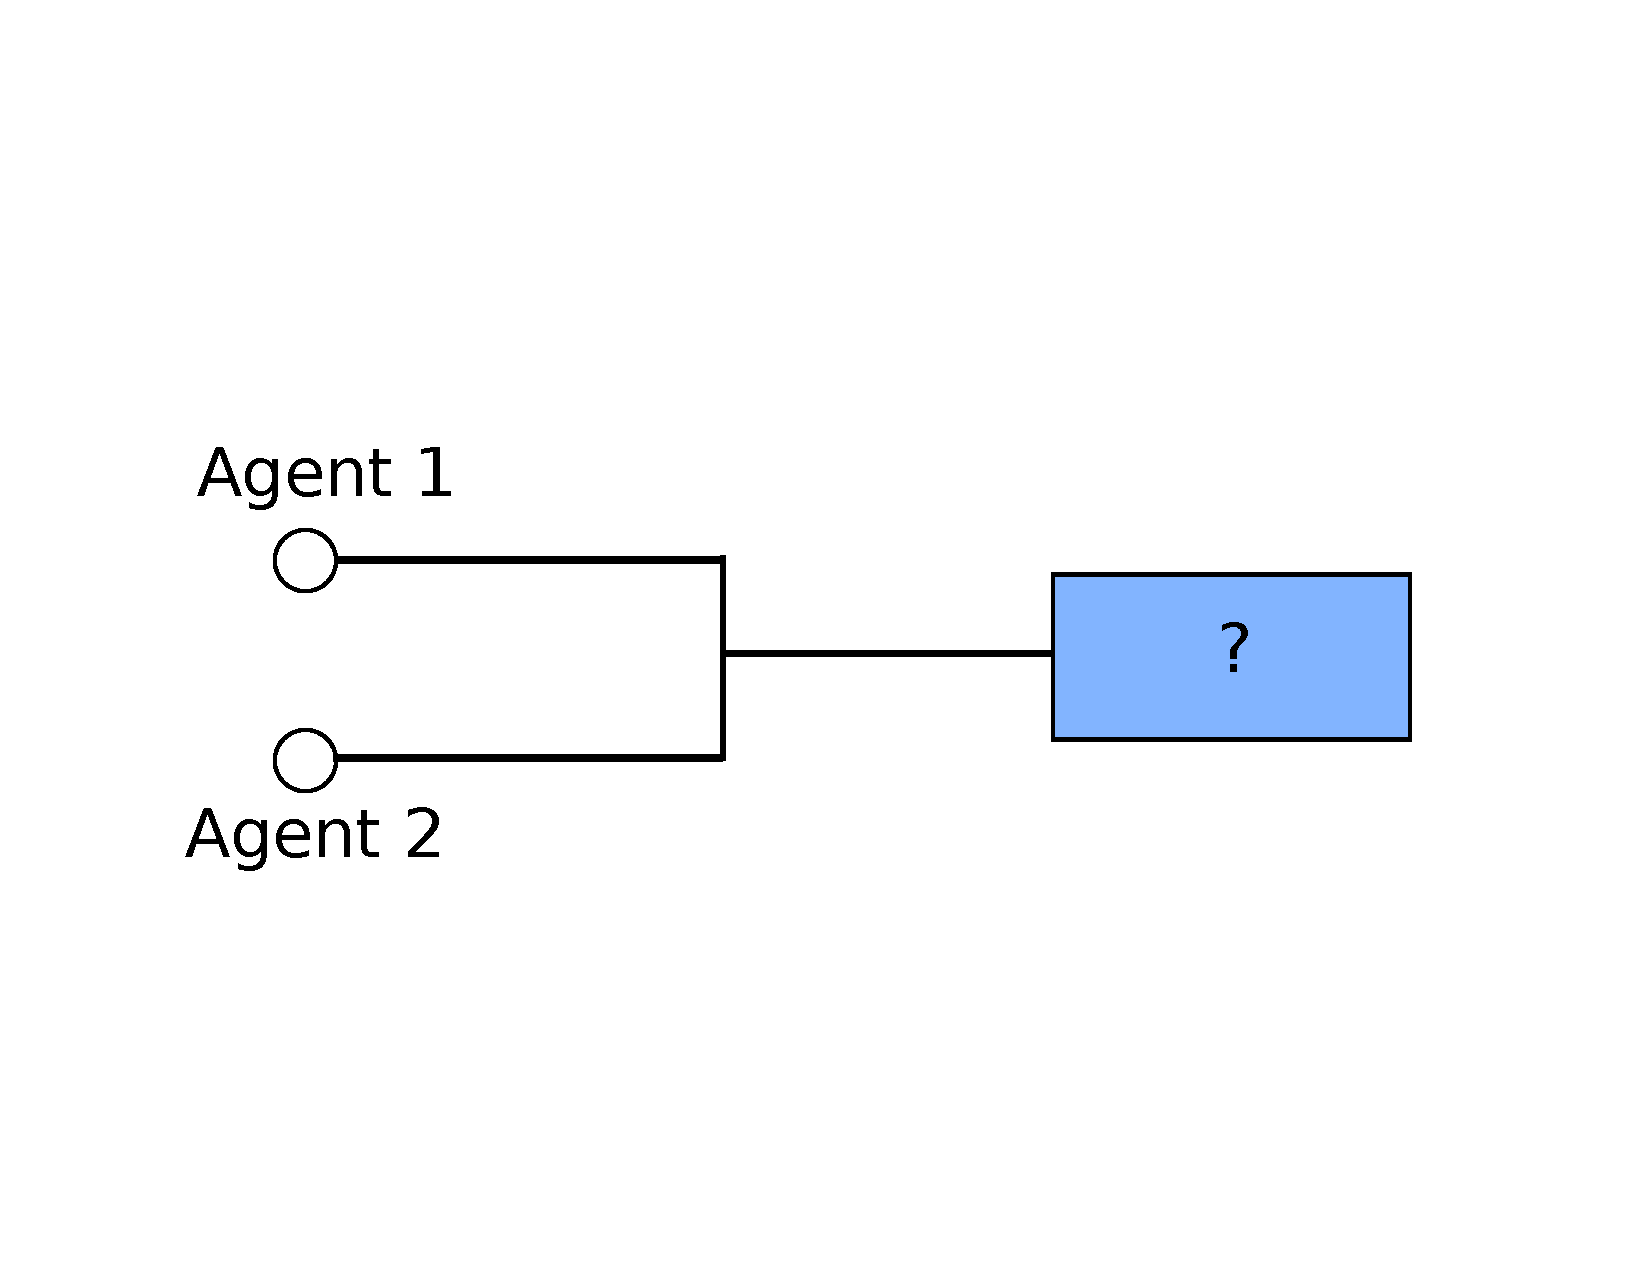
\includegraphics[scale=.3]{agents_ee}
	   \label{fig:agents_ee}
	\end{figure}
	\begin{itemize}
		\item The probability of an agent having a message to send is known.
		\item The reward for each agent sending a message is unknown in the
			planning stage.
	\end{itemize}
\end{frame}


\begin{frame}{Relevance}
	\begin{itemize}
		\item Several devices on a single internet connection (TV, telephone, PCs)
		\item For example:
		\begin{itemize}
			\item Emergency calls take priority
			\item Telephone calls always need a minimum of resources, but never
				the whole bandwidth
			\item Web browsing or gaming take priority over downloading large files
		\end{itemize}
	\end{itemize}
	\begin{figure}
		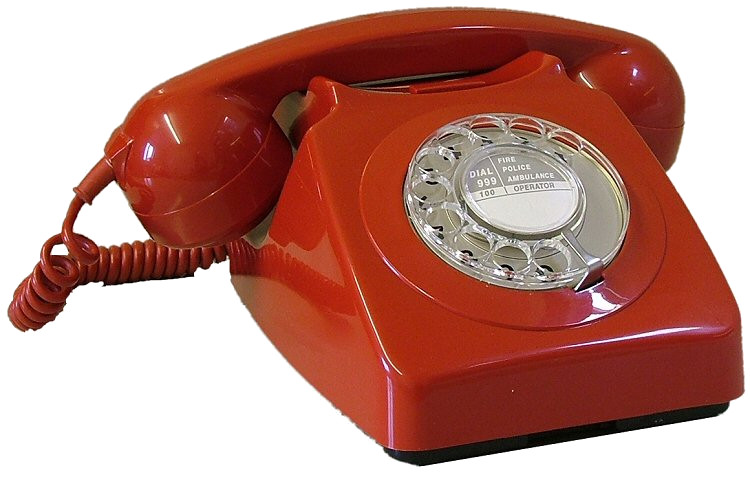
\includegraphics[height=5cm]{telephone}
	   \label{fig:telephone}
	\end{figure}
\end{frame}


\begin{frame}{Relevance}
	\begin{itemize}
		\item Prioritised load balancing in an operating system scheduler
		\begin{itemize}
			\item Increase responsiveness in consumer electronics
		\end{itemize}
		\item Efficiently sharing information over a single channel with multiple
			agents
	\end{itemize}
	\begin{figure}
		\caption{Agents sharing a single resource}
		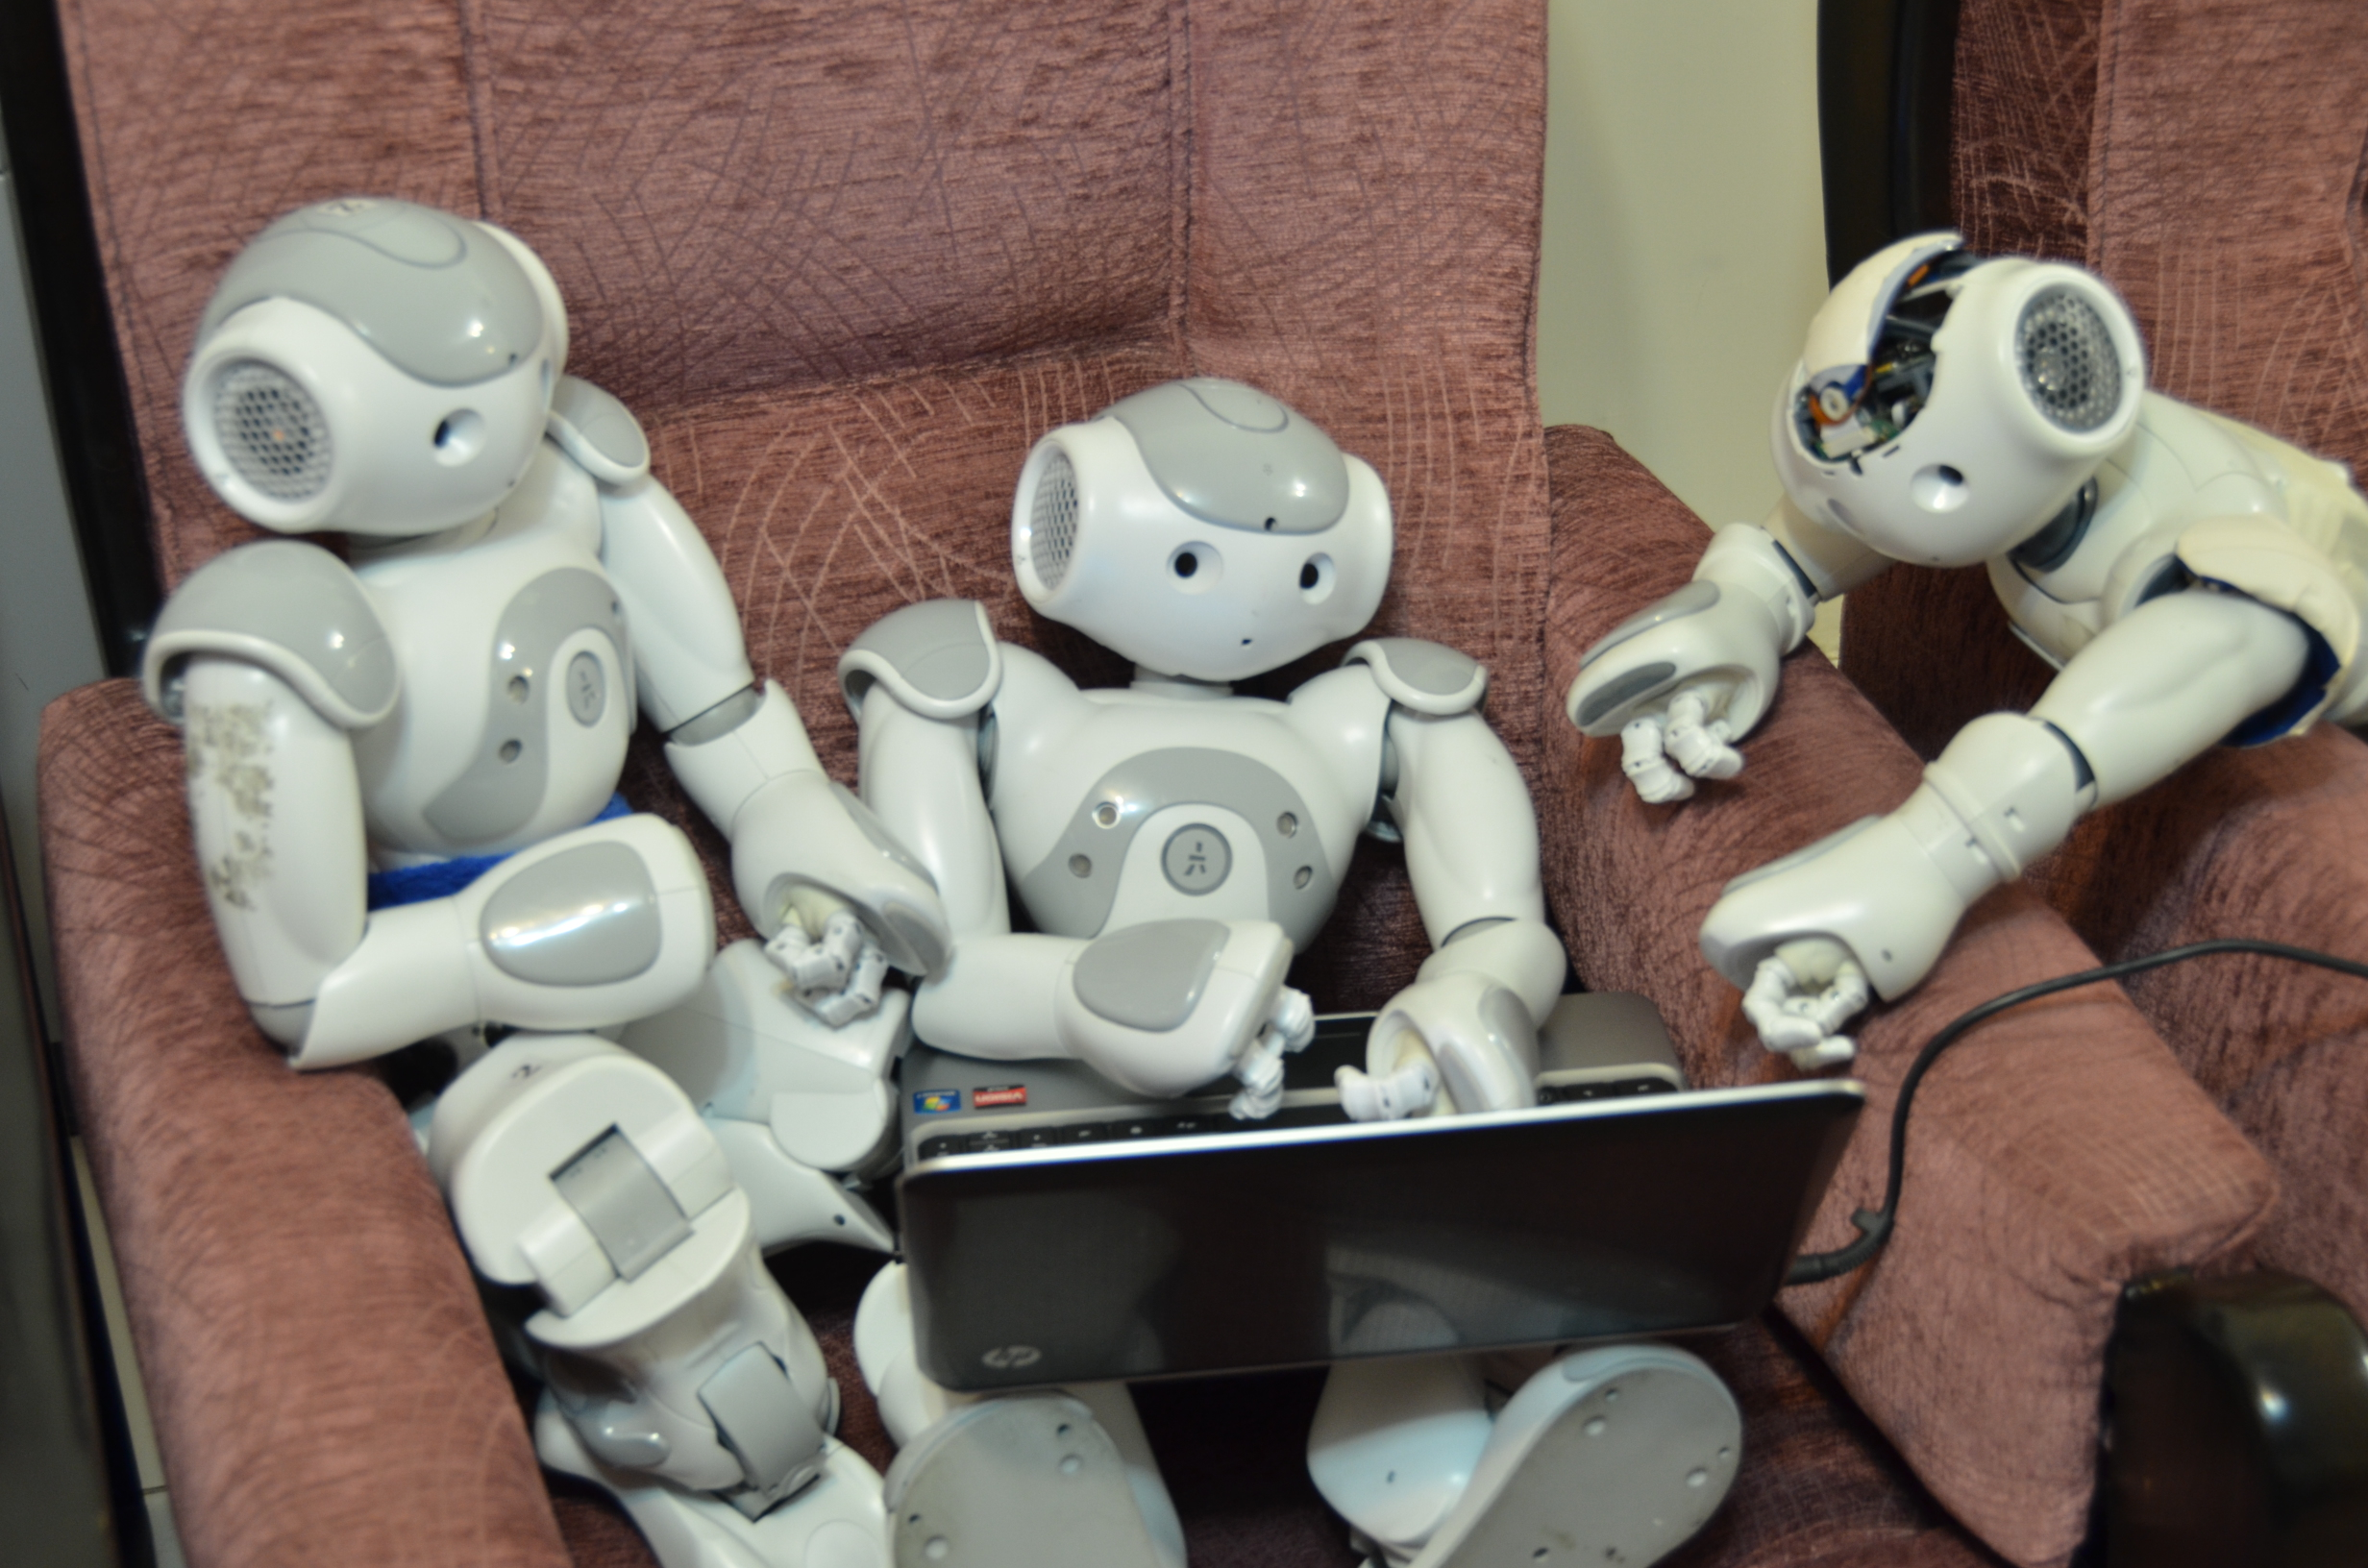
\includegraphics[height=5cm]{naos_pc}
	   \label{fig:naos_pc}
	\end{figure}
\end{frame}


\begin{frame}{Results}
	\begin{figure}
		\centering
		\begin{subfigure}[b]{0.3\textwidth}
			\centering
			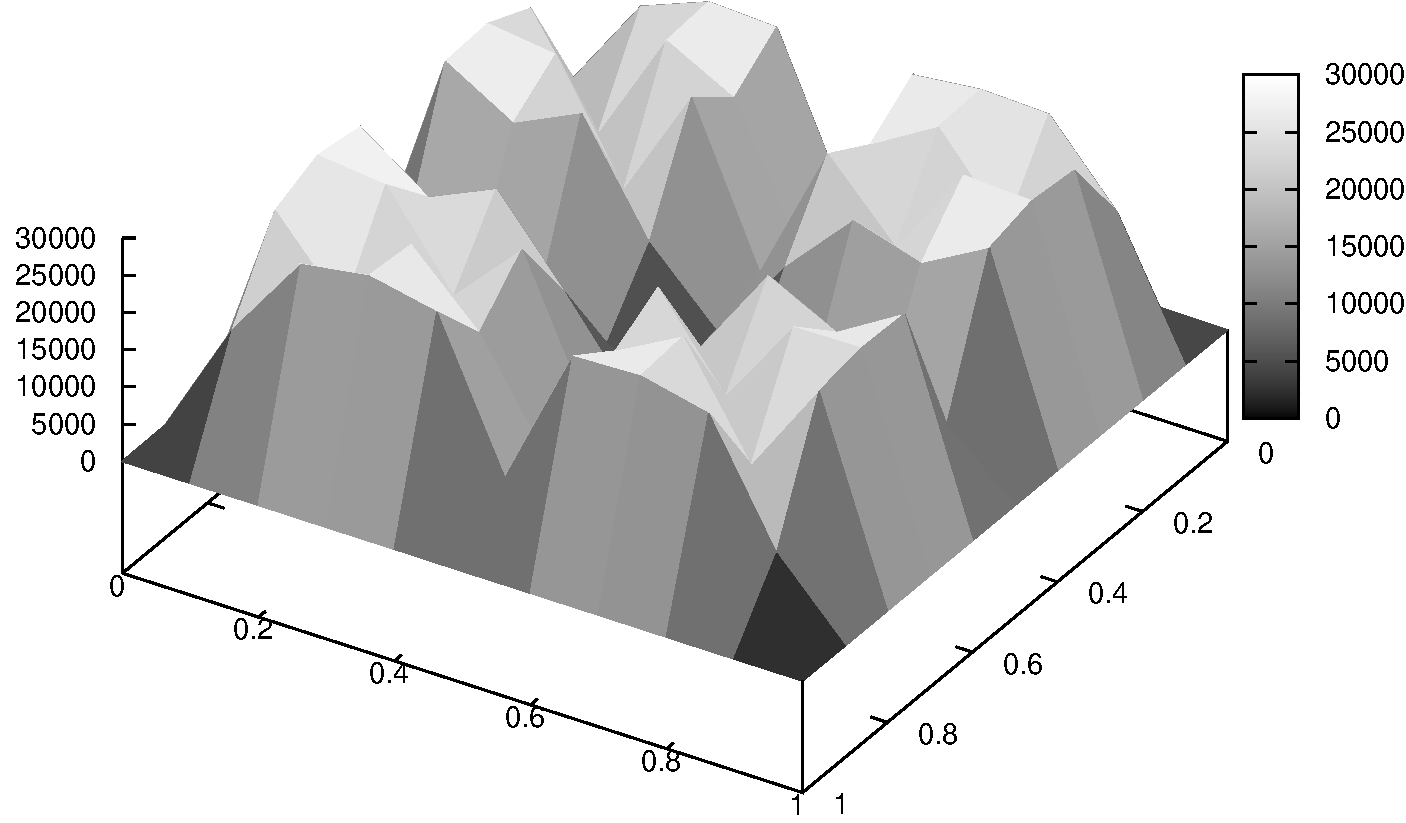
\includegraphics[height=2.5cm]{../../images/r3_nopareto}
			\caption{Without Pareto}
			\label{fig:../../images/r3_nopareto}
		\end{subfigure}
		\hspace{2cm}
		\begin{subfigure}[b]{0.3\textwidth}
			\centering
			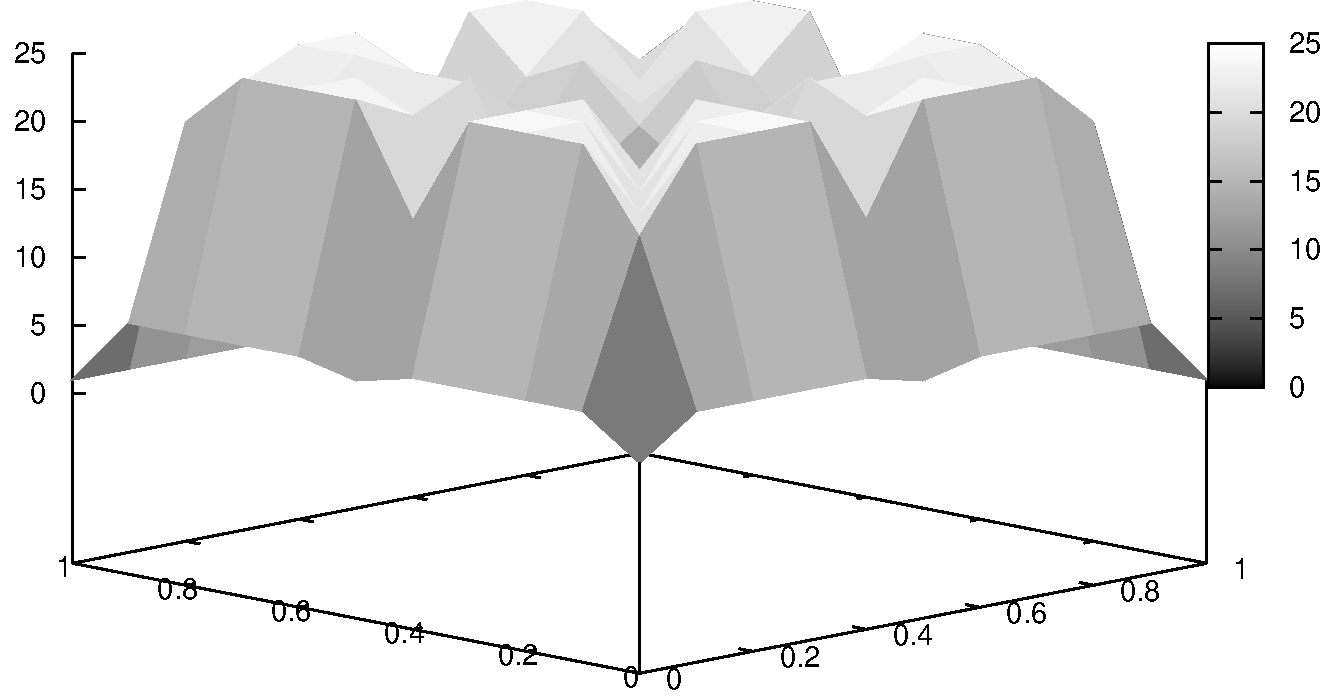
\includegraphics[height=2.5cm]{../../images/r3_diagonal}
			\caption{With Pareto}
			\label{fig:r3_diagonal}
		\end{subfigure}
		\caption{Reward set size}
	\end{figure}
	Set sizes differ only due to duplicate vectors All probability distributions
	benefit equally from Pareto optimisation (proportional to set size)
\end{frame}


\begin{frame}[Results]
	Pareto optimisation works (15 minutes to 4 seconds at 4 time steps for 2
	agents)
	\begin{figure}
		\centering
		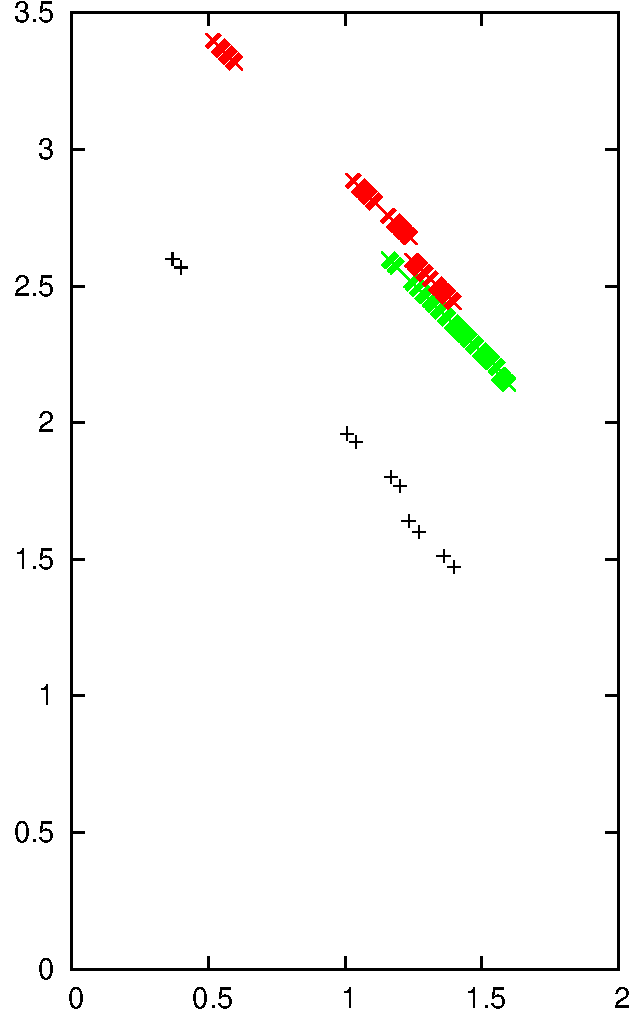
\includegraphics[height=5cm]{../../images/t4_28}
		\caption{Example of the Pareto set with probabilities 0.2 and 0.8 (t=4)}
		\label{fig:t4_28}
	\end{figure}
\end{frame}


\begin{frame}[Results]
	\begin{figure}
		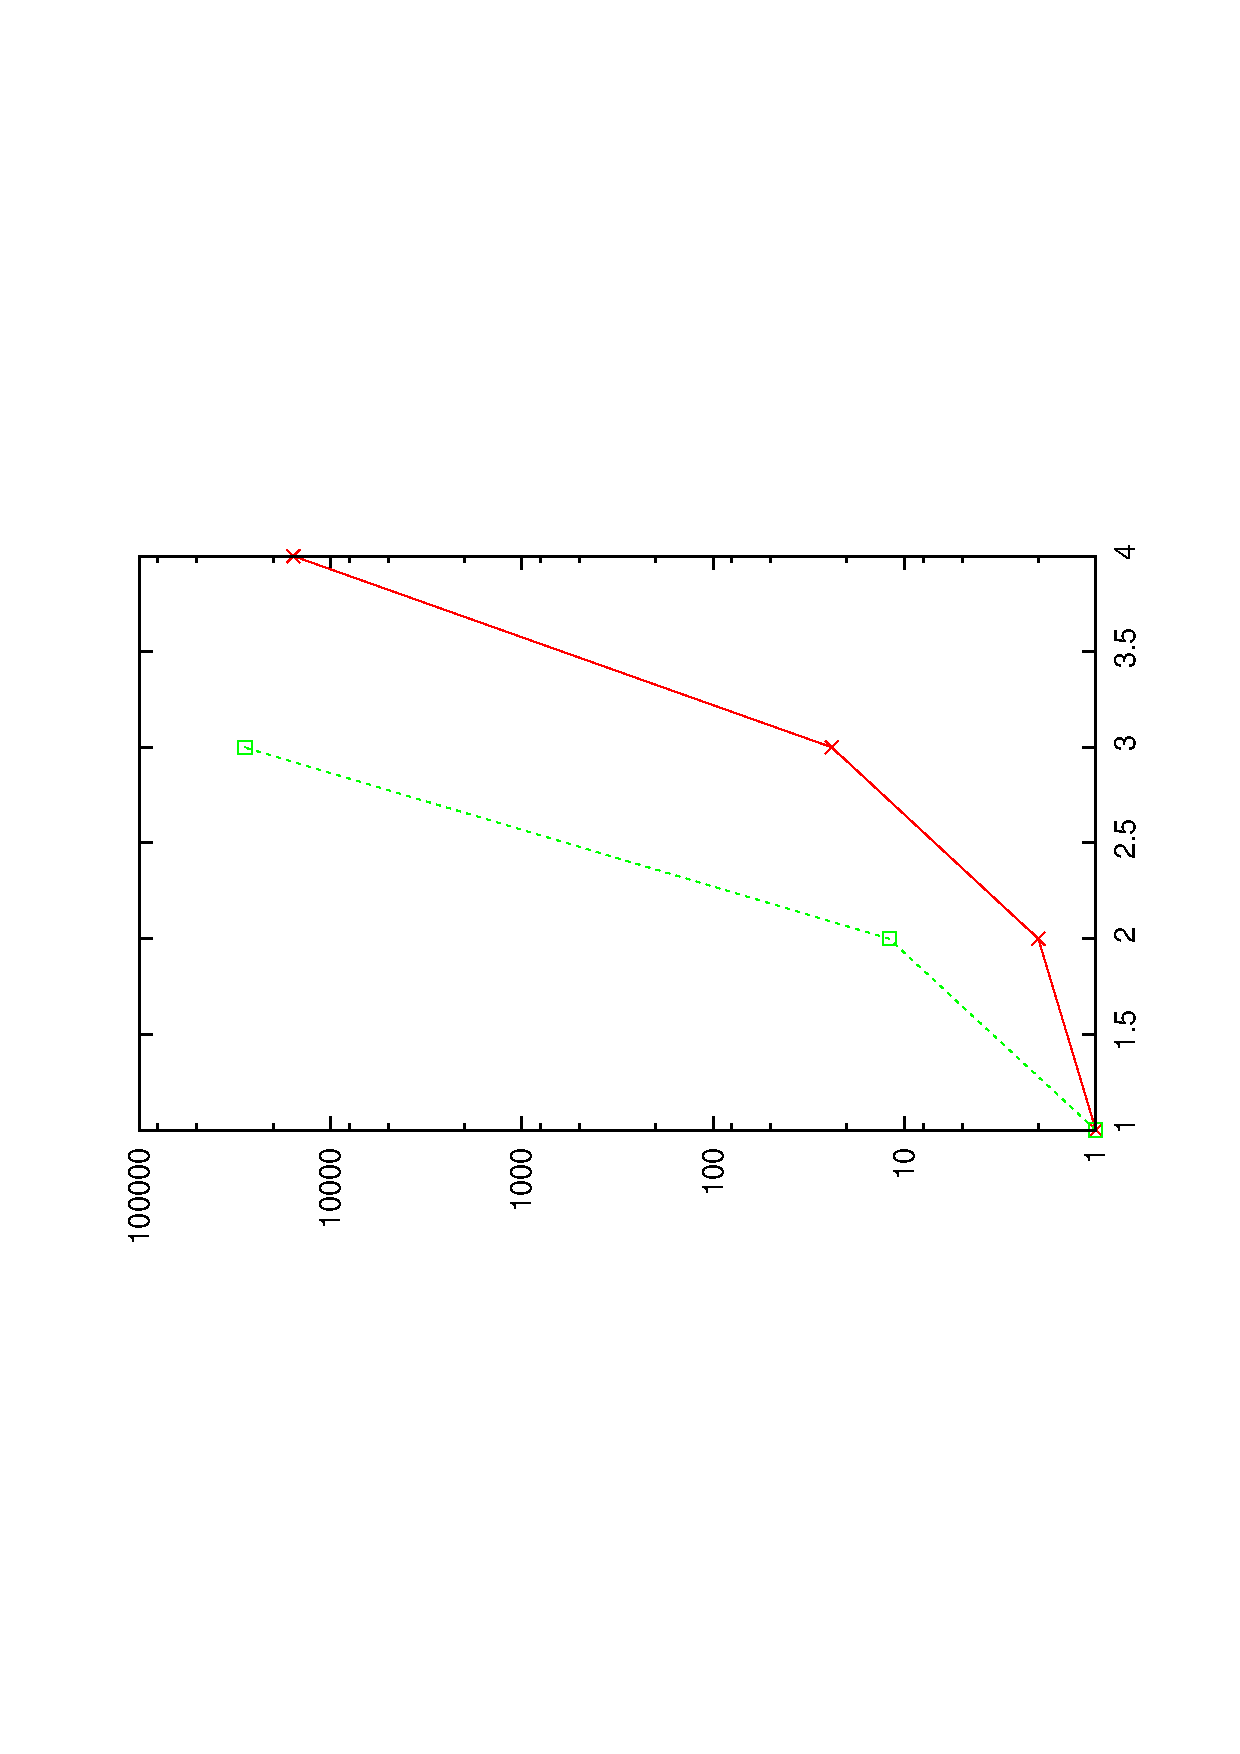
\includegraphics[scale=.3]{../../images/pareto_difference}
		\label{fig:../../images/pareto_difference}
		\caption{Size of Pareto-optimal set for number of time steps}
	\end{figure}
	Current implementation can not plan ahead more than 4 steps for 2 agents or
	2 for 3
\end{frame}

\begin{frame}[Future Research]
	\begin{itemize}
		\item Pareto-optimal sets are divided in hyperplanes perpendicular to the
			origin (memory space)
		\item Exploit C++ set structure: Adding new vector can rule out many
			other vectors (time complexity)
	\end{itemize}
\end{frame}
\end{document}
